\section{Background and Problem Statement } \label{sect:problem}

\subsection{TrustZone on ARM Cortex-M}

ARM TrustZone is a hardware-based security technology developed by ARM Holdings \cite{DemystifyingAT, TZArchitecture}. TrustZone essentially divides the ARM processor into two distinct execution environments: the ``Normal World'' and the ``Secure World''. In fact, this system-wide approach assigns two virtual cores to each physical processor, together with the mechanism to securely switch between both realms. These environments are isolated from each other, and the Normal World is typically where the non-secure, general-purpose operating system and applications run. The Secure World, on the other hand, is a more trusted and isolated area where security-critical operations, cryptographic functions, and sensitive data can be processed and stored.

On ARM application processors (Cortex-A) \cite{TZA}, a separate processor mode known as the secure monitor handles secure context switching between worlds. However, on ARM microcontrollers (Cortex-M) \cite{TZM} lack a dedicated secure monitor software. Instead, essential mechanisms integrated into the core logic act as gatekeepers, facilitating the transition between secure and non-secure realms. These two worlds are rigidly separated at the hardware level and possess differing levels of privilege. Non-secure software is explicitly restricted from directly accessing resources in the secure world. This chapter focuses exclusively on TrustZone features for Cortex-M processors.

TrustZone technology for Armv8-M devices is tailored for ARM microcontrollers, specifically the Cortex-M series. It's been finely tuned for swift context switching and ultra-low power embedded applications. Leveraging specialized hardware integrated into Cortex-M cores along with a dedicated secure instruction set, TrustZone facilitates the establishment of multiple software security domains. These domains enforce strict access controls, allowing trusted software exclusive access to secure memory and I/O, all while maintaining optimal system performance.

\textbf{Armv8-M Architecture} typically features a set of 32-bit general-purpose registers (R0 to R12, Link Register (LR), Program Counter (PC)) and floating-point register (D0-D15) that are shared between secure and non-secure states. TrustZone-enabled Armv8-M microcontrollers have separate stacks for each security state, with the Stack Pointer (SP) being security-banked, meaning one instance exists in each state. The CONTROL register and some other special-purpose registers are also banked, and the core automatically switches between their instances during state transitions. ARMv8-M architecture introduces a new ISA with additional instructions and features, which enhances code density, reduces interrupt latency, and improves system performance. The architecture includes a two-stage pipeline for instruction execution, providing efficient handling of instructions.

\textbf{Memory space} in the Armv8-M architecture is also partitioned into secure and non-secure memory regions. The secure memory space is further divided into two types: secure and non-secure callable (\ac{NSC}). Secure addresses are exclusively allocated for memory and peripherals that can only be accessed when the core is executing in secure state. The program address, the address of the instruction currently executed, determines the security state of the processor. In contrast, non-secure addresses are designated for memory and peripherals accessible by all software running on the device, including both secure and non-secure components. \ac{NSC} represents a unique class of secure memory locations that facilitates the transition of software from a non-secure to a secure state, allowing for controlled and secure state changes. 

The security state assigned to each memory address are established through either the programmable Secure Attribution Unit (\ac{SAU}) or by an fixed Implementation Defined Attribution Unit (\ac{IDAU}). The \ac{SAU} is always available in Armv8-M cores, while the \ac{IDAU} is external to the core and the presence depends on the vendors implementation. In cases where both the \ac{IDAU} and \ac{SAU} are available within a system, the \ac{SAU}'s attributions take precedence, unless the \ac{IDAU} specifies a higher security attribute for a particular address.The \ac{SAU} can only be programmed in the secure state. 

In ARM TrustZone-M, the Nested Vectored Interrupt Controller (NVIC) has been enhanced to enable secure and non-secure configuration for each interrupt. The processor seamlessly handles interrupts based on its current security state. Notably, when a non-secure interrupt occurs during secure code execution, the processor securely manages the transition, preserving secure context data and preventing information leakage.

For \textbf{Transition} between two worlds, three new instructions have been introduced including secure gateway (\ac{SG}), branch with exchange to non-secure state (\ac{BXNS}), and branch with link and exchange to non-secure state (\ac{BLXNS}). The \ac{SG} instruction is employed for switching from the non-secure to the secure state. It is typically found at the start of a secure entry point's veneer, which consists of an \ac{SG} instruction followed by a branch to the secure world's function. The veneers are meant to reside in memory regions attributed to the \ac{NSC} by the linker. The \ac{SG} instruction serves several functions, such as setting the security level to secure, banking registers, and resetting bit[0] of the LR register to 0, indicating that the return will lead to a transition back from secure to non-secure. To return from the secure world to the non-secure world, as illustrated in Fig. \ref{fig:Ttansition}, the compiler employs the \ac{BXNS} instruction. This instruction initiates a branch or return to the non-secure program.

\begin{figure}
  \centering
  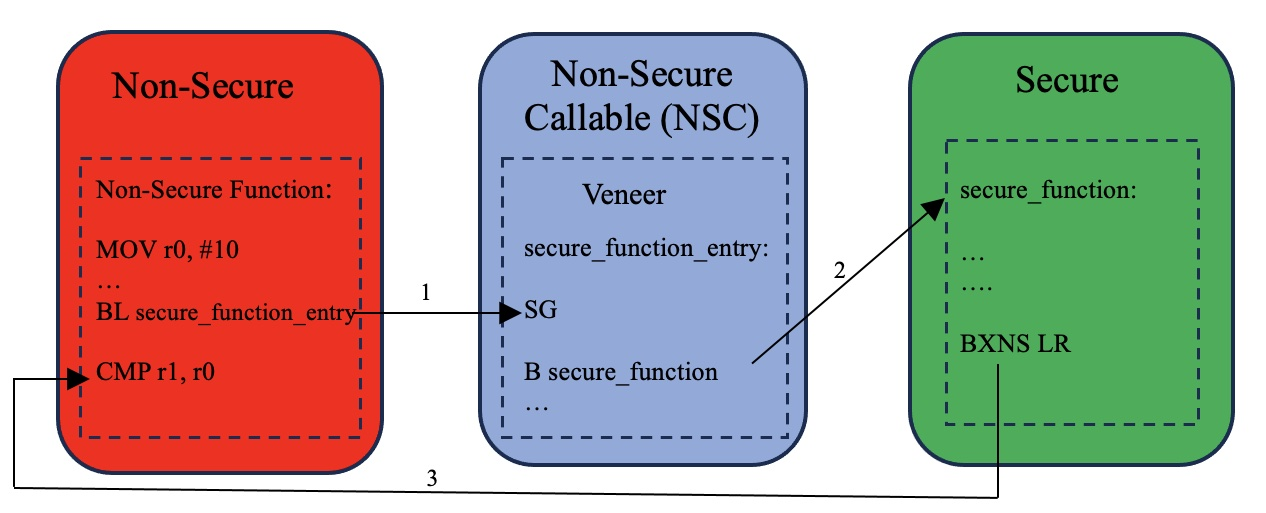
\includegraphics[width=\columnwidth]{figures/SFC.jpg}
  \caption{Secure Function Call in TrustZone-M}
  \label{fig:Ttansition}
\end{figure}

Conversely, secure software can invoke functions in the non-secure world. This action prompts the generation of compiler code that orchestrates the transition. It begins by preserving all registers, including the return address, within the secure stack. Subsequently, the registers are cleared. The \ac{BLXNS} instruction is used to execute the branch to the non-secure world, where it sets LR to a specific value, FNC\_RETURN (0xFEFFFFFF). Upon completion of the execution in the non-secure world, a return to the secure world is initiated using 'BX' instruction. When the BX instruction detects the FNC\_RETURN value in LR, it triggers a transition to the secure state. This shift is made possible by restoring all saved registers, including the return address, from the secure stack. It's also important to note that state transitions may also occur due to exceptions and interrupts.

TrustZone is not bullet-proof and has experienced successful attacks across various methods and contexts \cite{DemystifyingAT, surveyonTEE, returntononsecure}. The architecture, while designed to provide robust hardware-based security by isolating secure and non-secure worlds, is not immune to microarchitectural side-channel vulnerabilities \cite{DemystifyingAT, busted, surveyonTEE, truspy, Bypassed}. These vulnerabilities arise due to the shared resources and memory management between the secure and non-secure domains. Arm \cite{armdeveloper} has acknowledged that the security extensions for the Armv8-M architecture are not designed to protect against side-channel attacks resulting from control flow or memory access patterns. They argue that such attacks are not exclusive to the Armv8-M architecture and can apply to any code with secret-dependent control flow or memory access patterns. This type of attack can be mitigated by ensuring that the control flow and memory accesses patterns created by the program do not depend on secret state.

\subsection{Microarchitectural Side-Channel Attacks}

The security model proposed by \acp{TEE} is not foolproof and must be approached with caution regarding side-channel attacks. These attacks aim to uncover confidential information hidden within the shared microarchitectural state during a victim's execution by exploiting observable side effects, notably timing variations. Typically, adversaries begin by initializing the shared microarchitectural elements in a predetermined state. They then proceed to measure state changes during or after the victim's execution, utilizing methods such as transactional memory aborts or performance monitoring counters. However, the most prevalent method for observing microarchitectural state changes is through timing analysis \cite{vanbulckphdthesis}. In cases where microarchitectural optimizations depend on global stateful elements like Translation Lookaside Buffers (TLB), caches, or branch predictors, any modifications to these elements during the victim's execution will result in measurable timing differences in the attacker domain. The analysis of microarchitectural state updates provides valuable insights into the victim's behavior, even in scenarios where attackers are architecturally isolated and have limited interaction with the victim, strictly through defined input and output channels.

Single-purpose embedded processors typically emphasize simplicity, power efficiency, and cost-effectiveness over advanced microarchitectural features like caches, pipelining, and speculative execution. This focus results in predictable instruction timings, reducing the risk of side-channel attacks. However, research \cite{Travis, brumley2005remote} has demonstrated that secrets can still be revealed through start-to-end timing side channels, by measuring the overall execution time of secret-dependent branches, even on processors with entirely deterministic instruction timing behavior. 

In addition, Nemesis-type interrupt timing attacks \cite{Nemesis} can
exploit highly precise, instruction- granular timing measurements, which
can even compromise secrets from branches with balanced start-to-end
timings. These side-channel attacks abuse the CPU's interrupt mechanism to
reveal microarchitectural instruction timings within \acp{TEE}. The attack leverages the fact that hardware interrupts are only processed upon instruction retirement, after the currently executing instruction has completed, resulting in variable CPU cycles for different instruction types and processor states. Consequently, an untrusted operating system can precisely measure interrupt handling time, to retrieve the execution length of interrupted instruction and distinguish between secret-dependent program branches. In essence, for a successful Nemesis attack on processors with constant-time interrupt latency and multi-cycle instruction sets, where each instruction is uninterruptible, an attacker just requires a different execution time for at least one instruction in the if/else branch.

In recent findings, researchers have identified DMA-based side-channel
attacks specifically aimed at embedded TEEs \cite{busted, marton}. These
attacks exploit nuanced timing variations arising from contention between a
DMA device and the CPU as they access the shared memory bus. This
exploitation enables the attacker to construct a cycle-accurate memory
access trace of a victim program. Notably, at the Black Hat Asia
conference, Cristiano Rodrigues presented a side-channel attack that
leverages DMA to target ARM TrustZone. This sophisticated attack
effectively bypasses hardware-enforced isolation primitives, providing
unauthorized access to Trusted Applications (\acp{TA}) and resulting in the unauthorized leakage of sensitive information.

\subsection{BUSted: Microarchitectural Side-Channel Attacks on TrustZone-M MCUs}

BUSted \cite{busted} is a novel class of microarchitectural side-channel attacks that leverage the timing differences exposed in the arbitration logic of the MCUs bus intecconnect. It's evident that concurrent access by multiple bus master (e.g., CPU, DMA) to a shared bus slave (e.g., memory controller) leads to time delays for at least one, causing subtle timing variations. By observing the timing drifts on memory transactions, an attacker can extract information regarding the victim’s memory access pattern. Consequently, without breaking security isolation boundaries, a malicious bus master can spy on bus activity and determine when another bus master accessed a specific slave.

ARM adopts a load-store memory access model, restricting memory interaction solely to load/store (LDR and STR) instructions. Thus, an attacker can exploit the MCU's load-store architecture to observe timing variations. Specifically, in cases where the victim code incorporates secret-dependent control flow and loads/stores execute at different clock offsets on conditional paths, this discrepancy leads to distinct memory access patterns. An attacker could exploit this to deduce and illicitly obtain a particular secret.

To elaborate further, let's examine a code snippet (compiled for the Arm Cortex-M23) that includes a balanced conditional statement dependent on a secret variable, as visualized in Fig. \ref{fig:busted}. Since both execution paths have an identical execution time of 5 clock cycles, starting from t + 1 after the \textit{cmp} instruction, an attacker wouldn't observe any difference in execution time. Consequently, distinguishing between these execution paths and subsequently extracting the secret becomes unfeasible. Yet, an observer could still detect divergent memory access patterns between these two execution paths. When the branch (\textit{bne}) isn't taken, it completes within a single clock cycle, causing the \textit{str} instruction to occur at clock cycle t + 3. Conversely, if taken, the branch incurs a two-clock-cycle process, resulting in the \textit{str} instruction taking place at clock cycle t + 4. Overall, this changes the relative position of the \textit{str} instruction to the \textit{bne} instruction and unveils the secret. By monitoring either 't + 3' or 't + 5' clock cycles, an attacker can potentially deduce the secret by observing the presence or absence of contention on the data memory bus.

\begin{figure*}
  \centering
  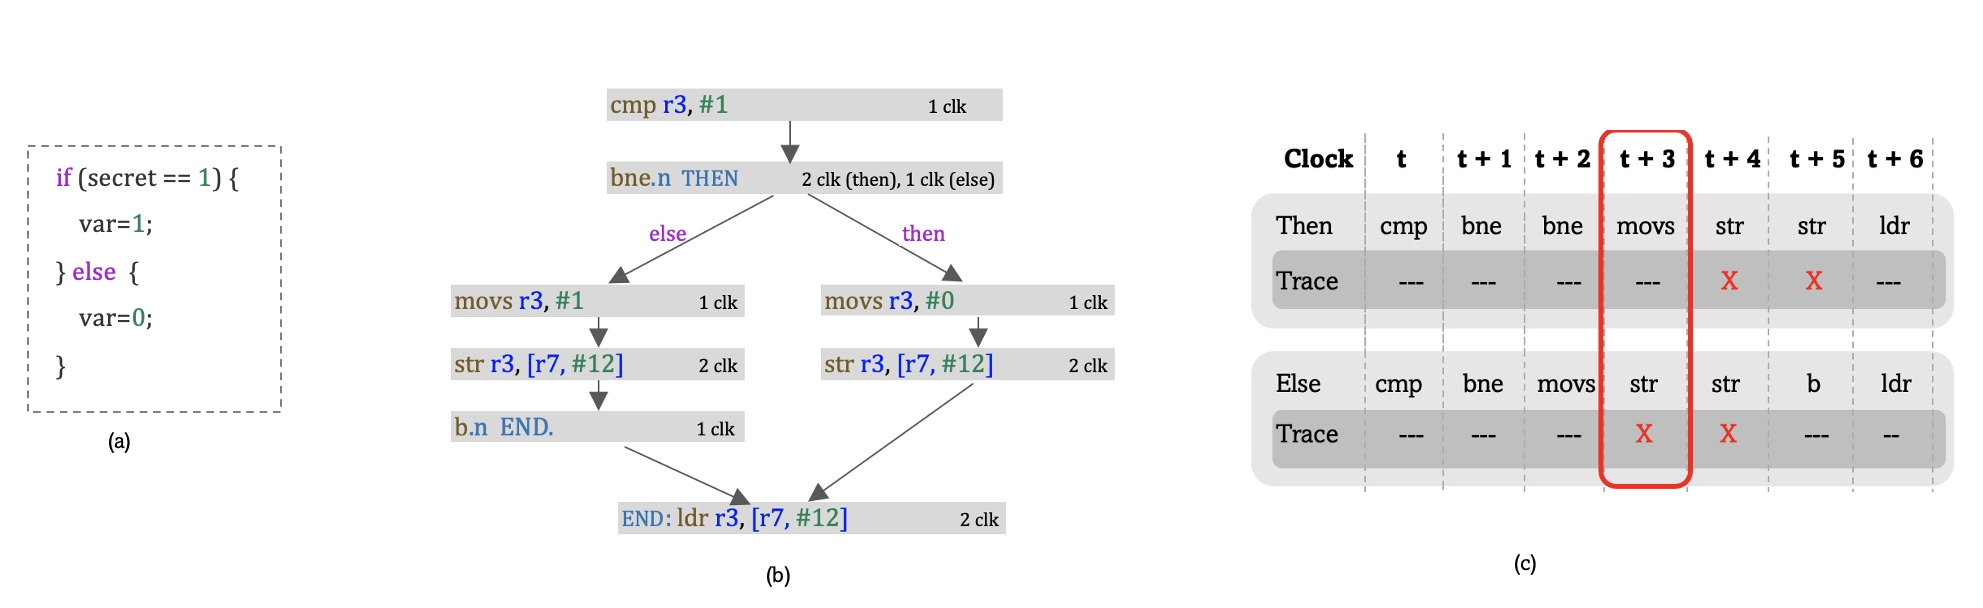
\includegraphics[width=\textwidth]{figures/busted.jpg}
  \caption{(a) secret-dependent branch, (b) compiled code CFG for Arm Cortex-M23, (c) memory access pattern and monitoring of clock t+3 and t+5.}
  \label{fig:busted}
\end{figure*}

Given the nature of this attack, targeting on microarchitectural design issues, comparisons have arisen likening its impact to that of renowned exploits like 'Spectre' and 'Meltdown' which affected more complex architectures in recent history. Embedded projects relying on hardware-assisted privilege separation via TrustZone-M must now factor in the potential for information leakage from secure components operating within the secure world. According to the researchers, there are software-based countermeasures available to mitigate the impact of this microarchitectural design flaw. The crucial consideration in addressing time-based attacks involves minimizing the presence of secret-dependent code in security operation implementations. Essentially, the time required for a security procedure should remain independent of the success or any secret of the operation.

\subsection{Covert Storage Channels}

Sensitive information can be unintentionally leaked through covert storage channels \cite{storagechannel, sabelfeld}. These channels, whether explicit or implicit, provide pathways for the unauthorized transfer of sensitive data, which can compromise system security. Implicit covert storage channels, in particular, introduce challenges, as data can inadvertently traverse indirect or unintended pathways resulting from the program's control structure. This contrasts with explicit information flows, which occur when confidential data is directly assigned to public variables. To illustrate, let us consider a scenario with two security levels: ``high'' and ``low,'' denoting varying degrees of confidentiality. We can examine the code presented in Fig. \ref{fig:implicit}, which exhibits a data flow from the high variable \textit{h} to the low variable \textit{l}. The insecurity within this code stems from the \textit{l = 1} assignment in a control context conditioned upon the confidential variable \textit{h}.

\begin{figure}
  \centering
  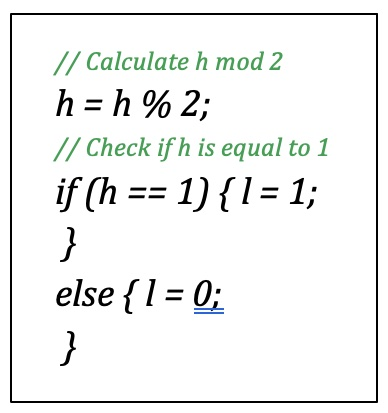
\includegraphics[width=.5\columnwidth]{figures/implicit.jpg}
  \caption[Short caption for Table of Figures]{An implicit information flow}
  \label{fig:implicit}
\end{figure}

\subsection{Static Code Analysis}

\textbf{Taint Analysis} stands as a crucial program analysis method, meticulously tracing the flow of data of interest throughout program execution. Taint analysis utilizes 'taint tags' as markers attached to registers and memory, serving to indicate their taint status. It operates via three integral components:

\begin{enumerate}
  \item[1.] Taint Sources: These denote points within the program or memory locations where relevant data is introduced, often focusing on user inputs from local or remote sources.
  
  \item[2.] Taint Propagation: This involves the transfer of taint tags during program execution, governed by predefined rules aligned with instruction semantics. Consider the instruction ADD src, dst; in this scenario, a taint propagation rule might dictate that the resulting tag of destination (dst) comprises a bitwise OR operation between the tags associated with src and dst.
  
  \item[3.] Taint Sinks: These specific program instructions serve as checkpoints for taint analysis, assessing the presence of targeted taint tags. They play a critical role in security applications, detecting potential threats like control flow hijacks or information leaks, often associated with control flow transfers or output system calls.
  
\end{enumerate}

\textbf{Value Set Analysis} operates as a static program analysis technique, approximating the potential values that each program data object might hold at any given program point. By analyzing individual instructions within a control-flow graph (CFG), value set analysis effectively tracks and estimates the diverse range of values that each data object could hold. 

\textbf{Symbolic Execution} stands as a method to explore the potential paths of program execution by substituting variables with symbolic representations. It systematically traverses the program, executing with symbolic inputs to understand the possible behaviors and identify vulnerabilities or paths that might lead to critical issues.
